%        File: pnas1.tex
%     Created: Wed Apr 30 04:00 pm 2014 E
% Last Change: Wed Apr 30 04:00 pm 2014 E
%
\documentclass[letterpaper]{article} 
\usepackage{caption} 
\usepackage{aaai} 
\usepackage{times} 
\usepackage{helvet} 
\usepackage{courier} 
\setlength{\pdfpagewidth}{8.5in} 
\setlength{\pdfpageheight}{11in} 
%%%%%%%%%%
% PDFINFO for PDFLATEX
% Uncomment and complete the following for metadata (your paper must compile with PDFLATEX)
\pdfinfo{
	/Title Inter-Task Effects induce Bias in Crowdsourcing
	/Author Edward Newell
	/Keywords priming, framing, micro-task, crowdsourcing
}


\usepackage{graphicx}
\usepackage{amsmath}
\usepackage{amssymb}
\usepackage{mathrsfs}
\usepackage{gensymb}
\usepackage{algorithm2e}
\usepackage{amsthm}

\newtheorem*{mydef}{Definition}

\usepackage{framed, color}
\usepackage{soul}
\usepackage[colorlinks=false, urlcolor=blue]{hyperref}
\usepackage{dcolumn}
\usepackage{multirow}
\usepackage{booktabs}
\newcolumntype{d}{D{.}{.}{4.0}}
\newcolumntype{s}{D{.}{.}{1.4}}

%\setlength{\parindent}{0cm}
%\setlength{\parskip}{4mm plus1mm minus1mm}

%%%%%%%%%%
% Section Numbers
% Uncomment if you want to use section numbers % and change the 0 to a 1 or 2
% \setcounter{secnumdepth}{0} %%%%%%%%%%
\title{Inter-Task Effects induce Bias in Crowdsourcing}
\author{Edward Newell\footnote{bla} \and Derek Ruths\\
School of Computer Science, McGill University, Montreal, Canada\\
$^*$\texttt{edward.newell@mail.mcgill.ca}\\
}
%%%%%%%%%%
% Body of Paper Begins
\begin{document}
\begin{figure*}
	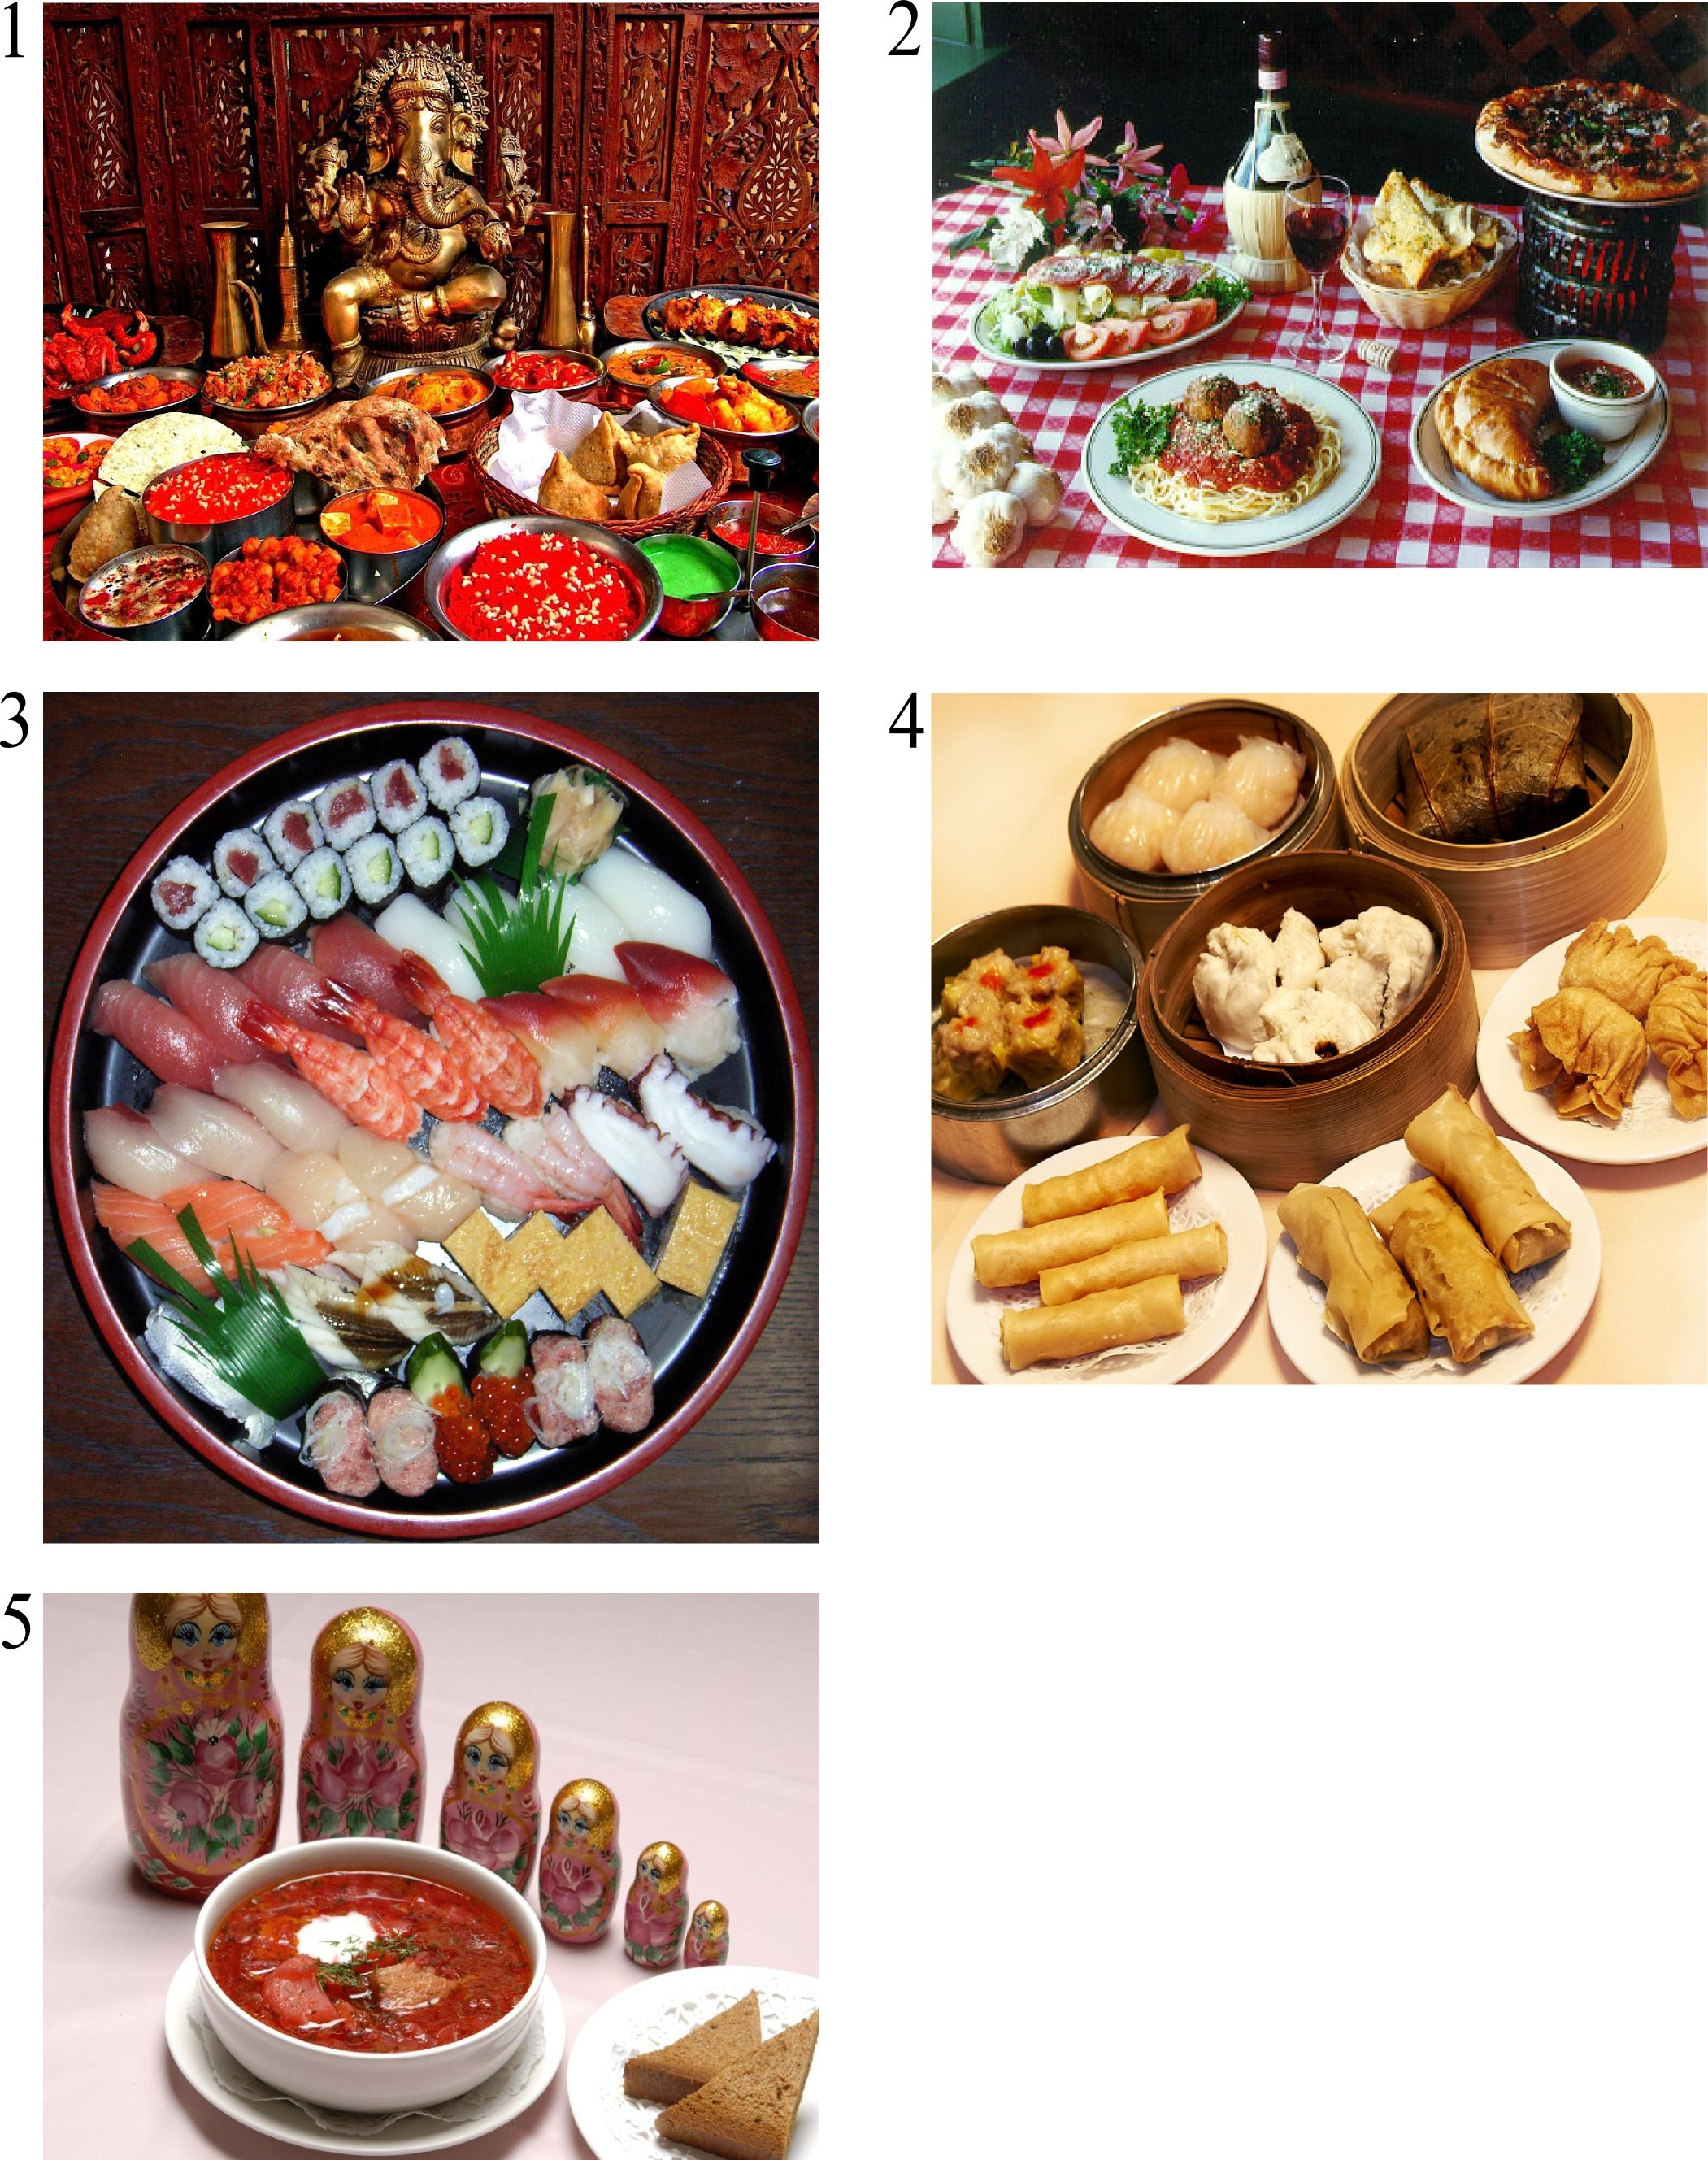
\includegraphics[scale=1.00]{figs/taskImages/testImages.jpg}
	\caption*{Figure S1: Testing image set. These images were presented to all workers in 
		the order shown after the initial set of images.}
\end{figure*}

\begin{figure*}
	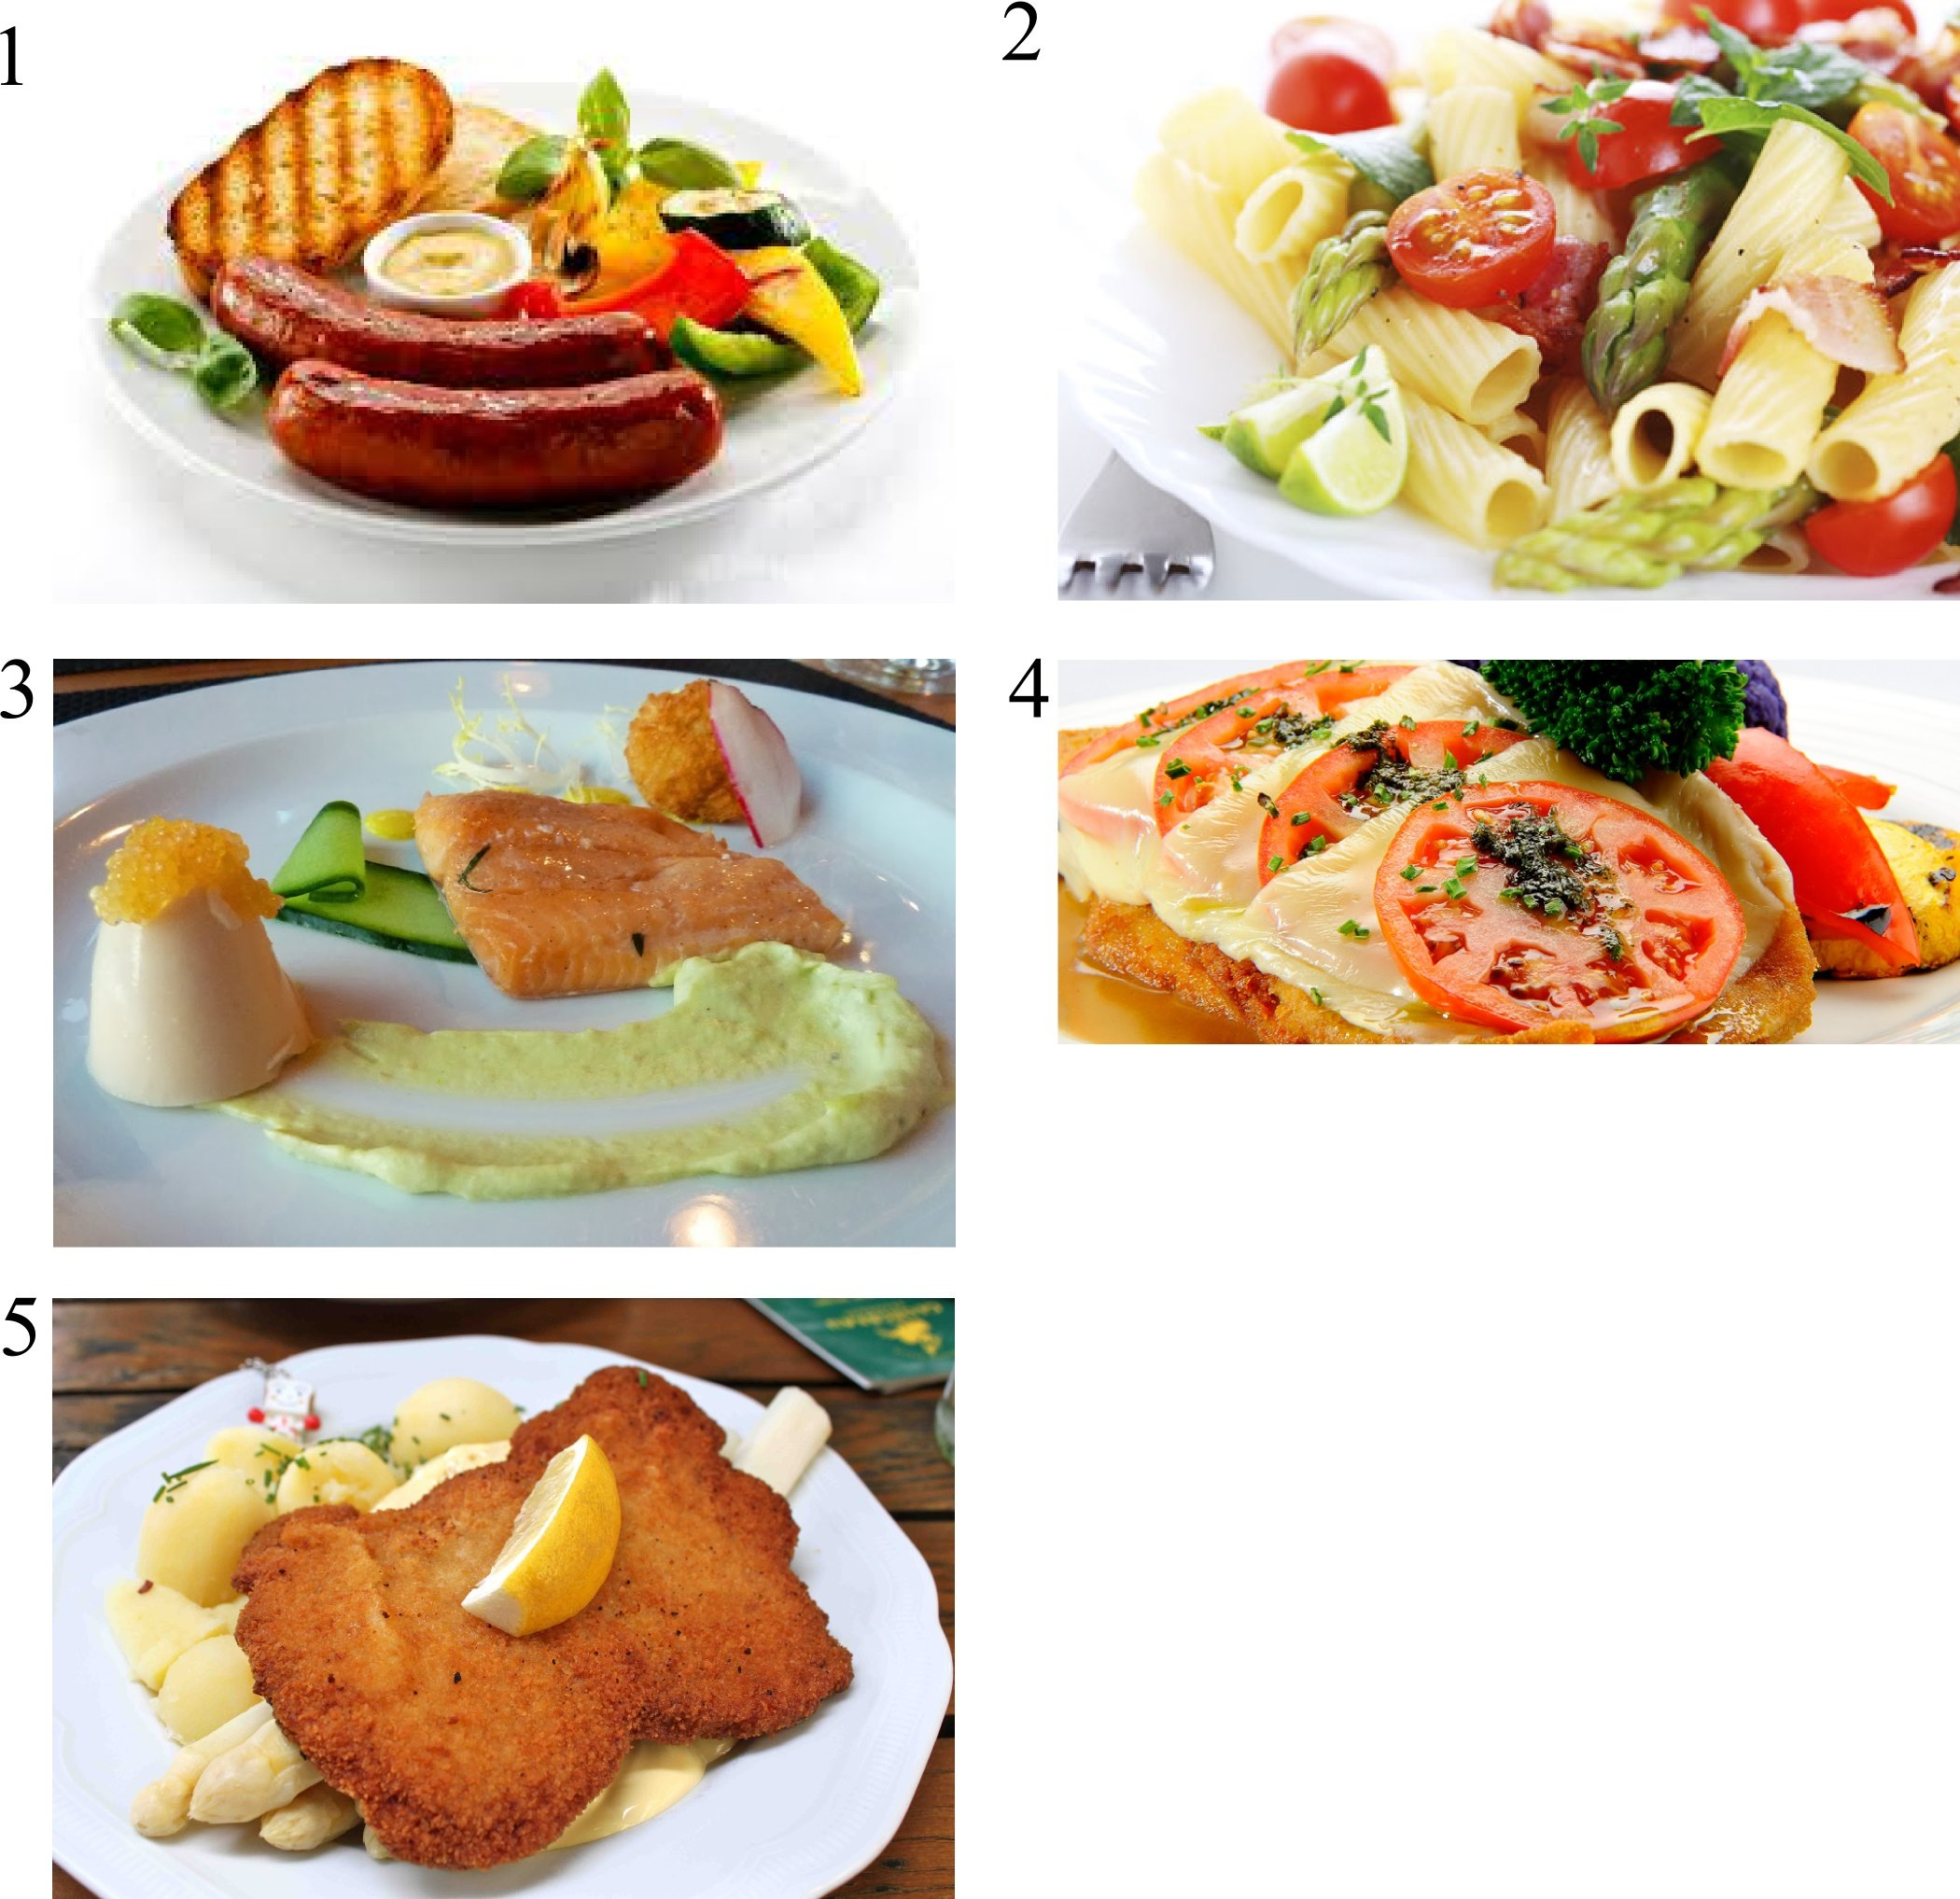
\includegraphics[scale=1.00]{figs/taskImages/ambiguous.jpg}
	\caption*{Figure S2: Ambiguous image set. These images were presented to workers from 
		certain treatments (see \textbf{Table 1}) in the main text.}
\end{figure*}

\begin{figure*}
	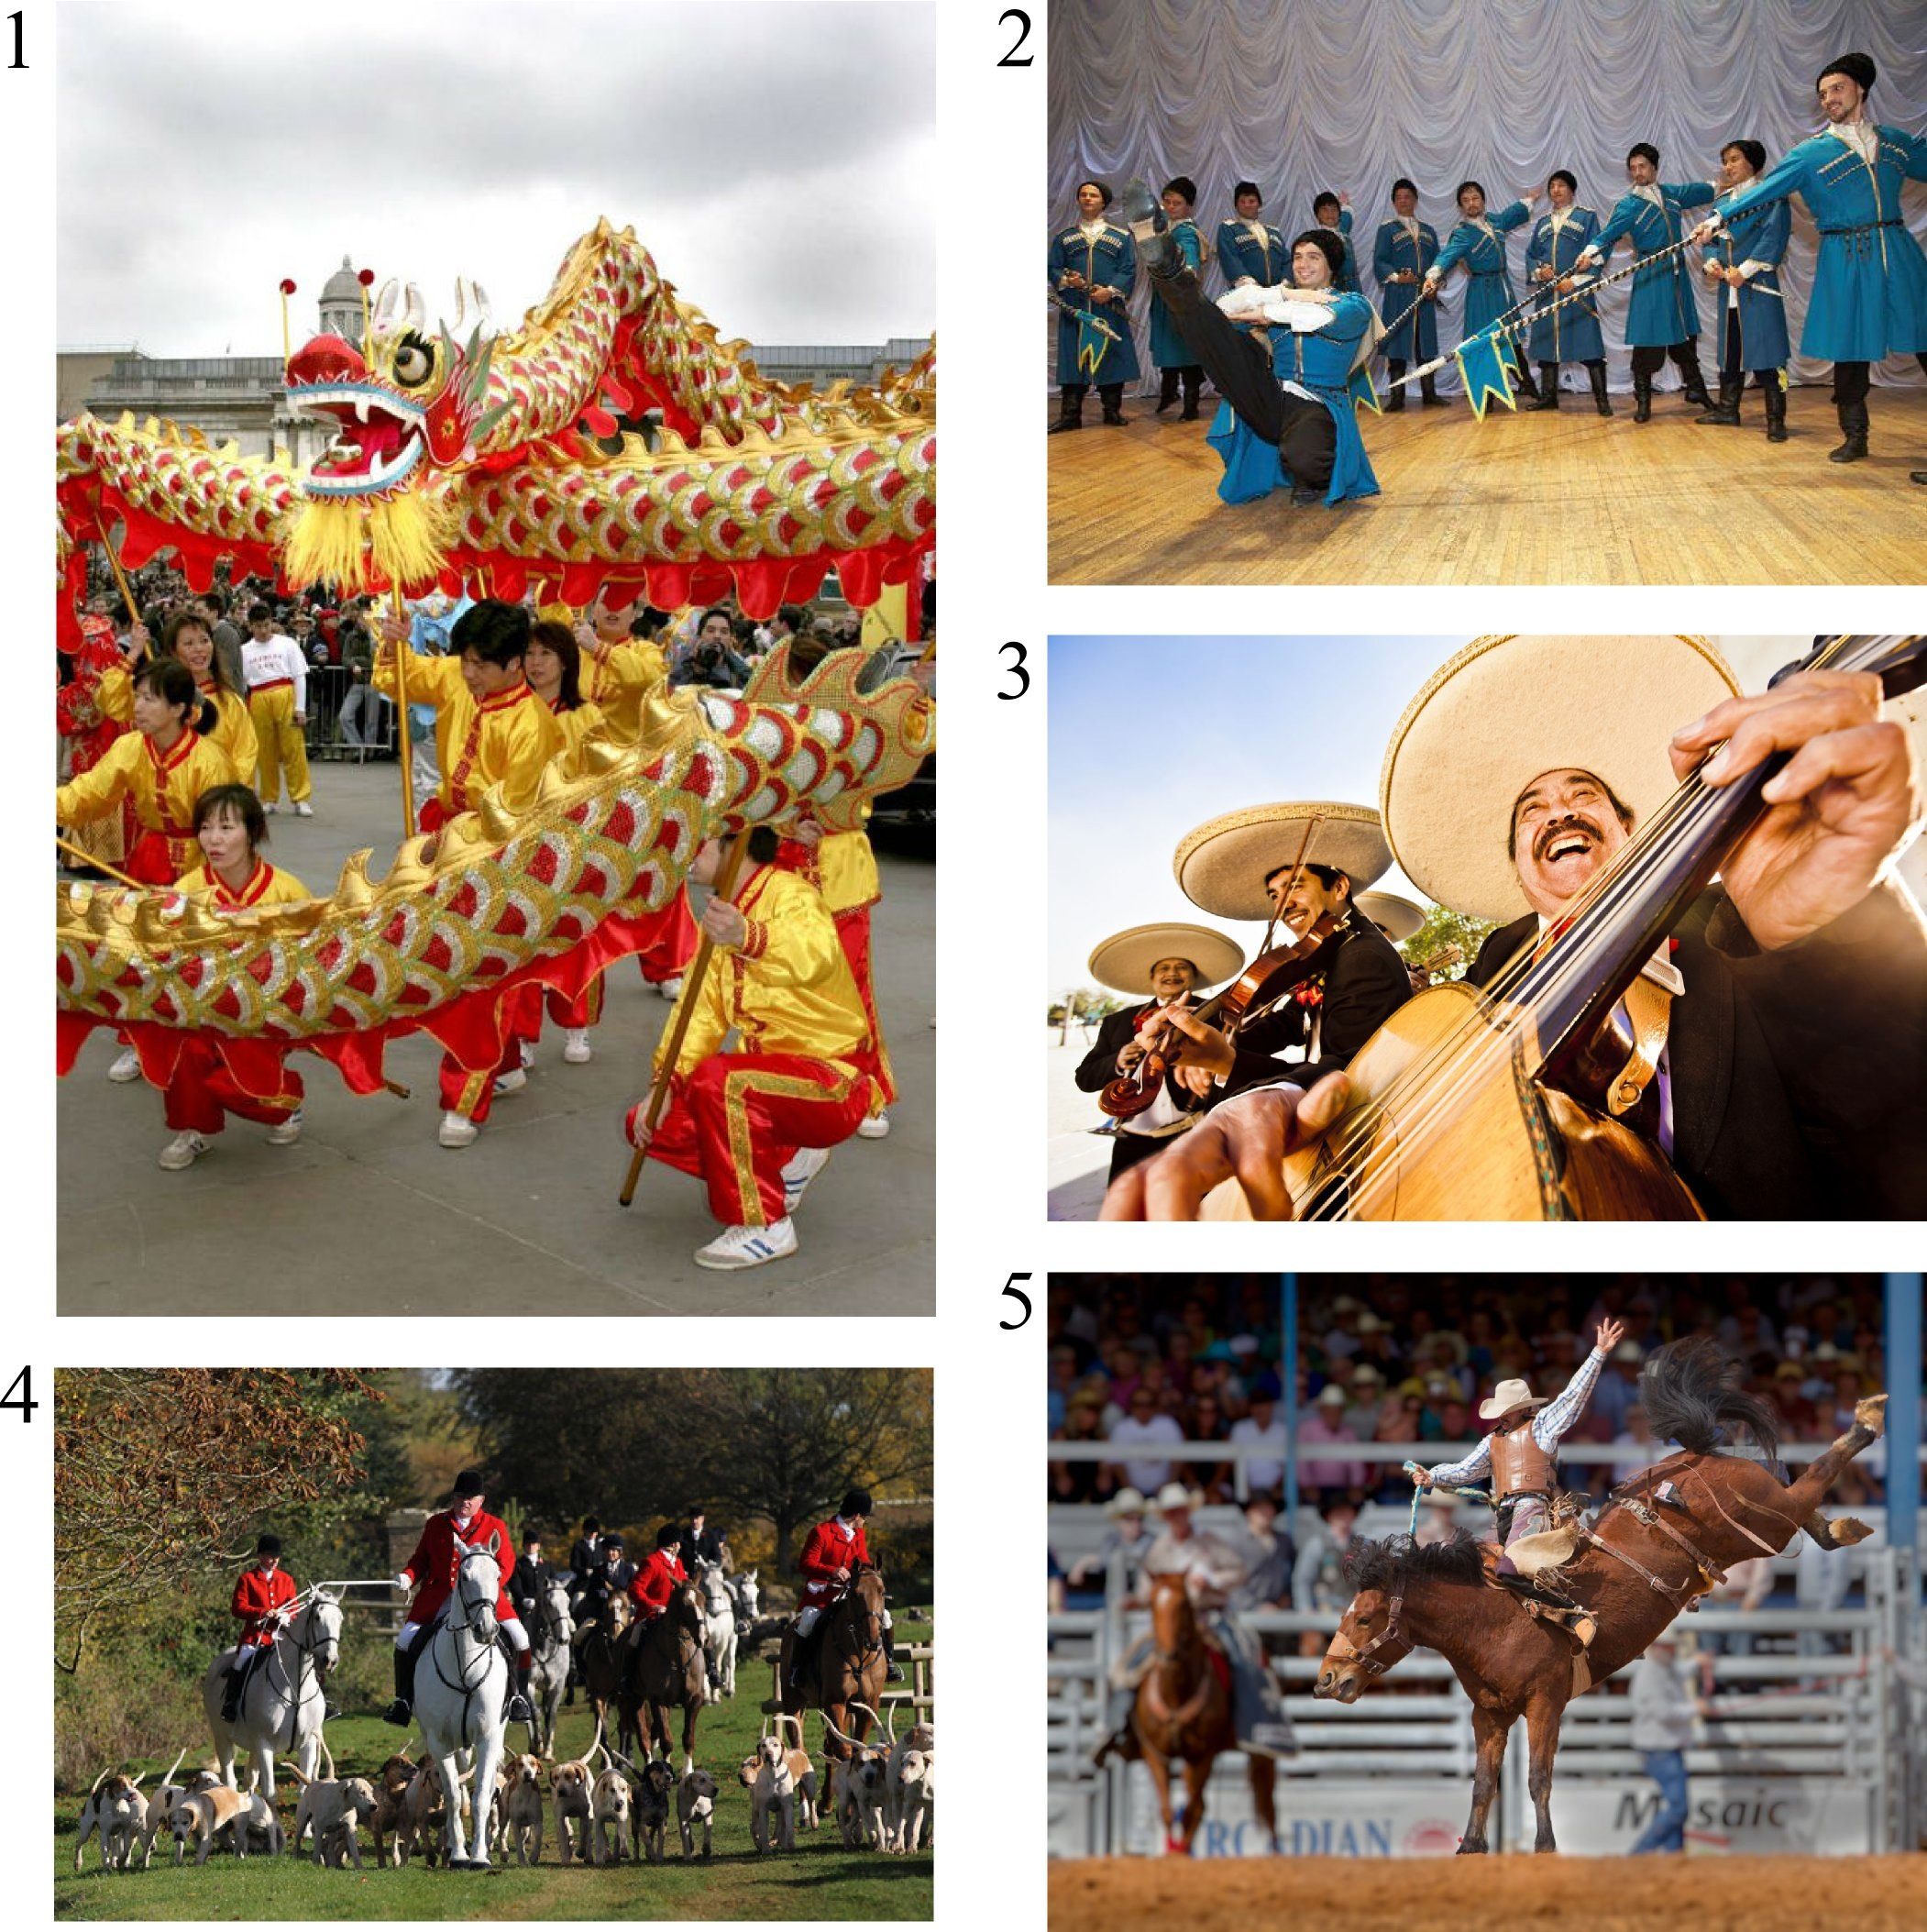
\includegraphics[scale=1.00]{figs/taskImages/cultural.jpg}
	\caption*{Figure S3: Cultural image set. These images were presented to workers from 
		certain treatments (see \textbf{Table 1}) the main text.}
\end{figure*}

\begin{figure*}
	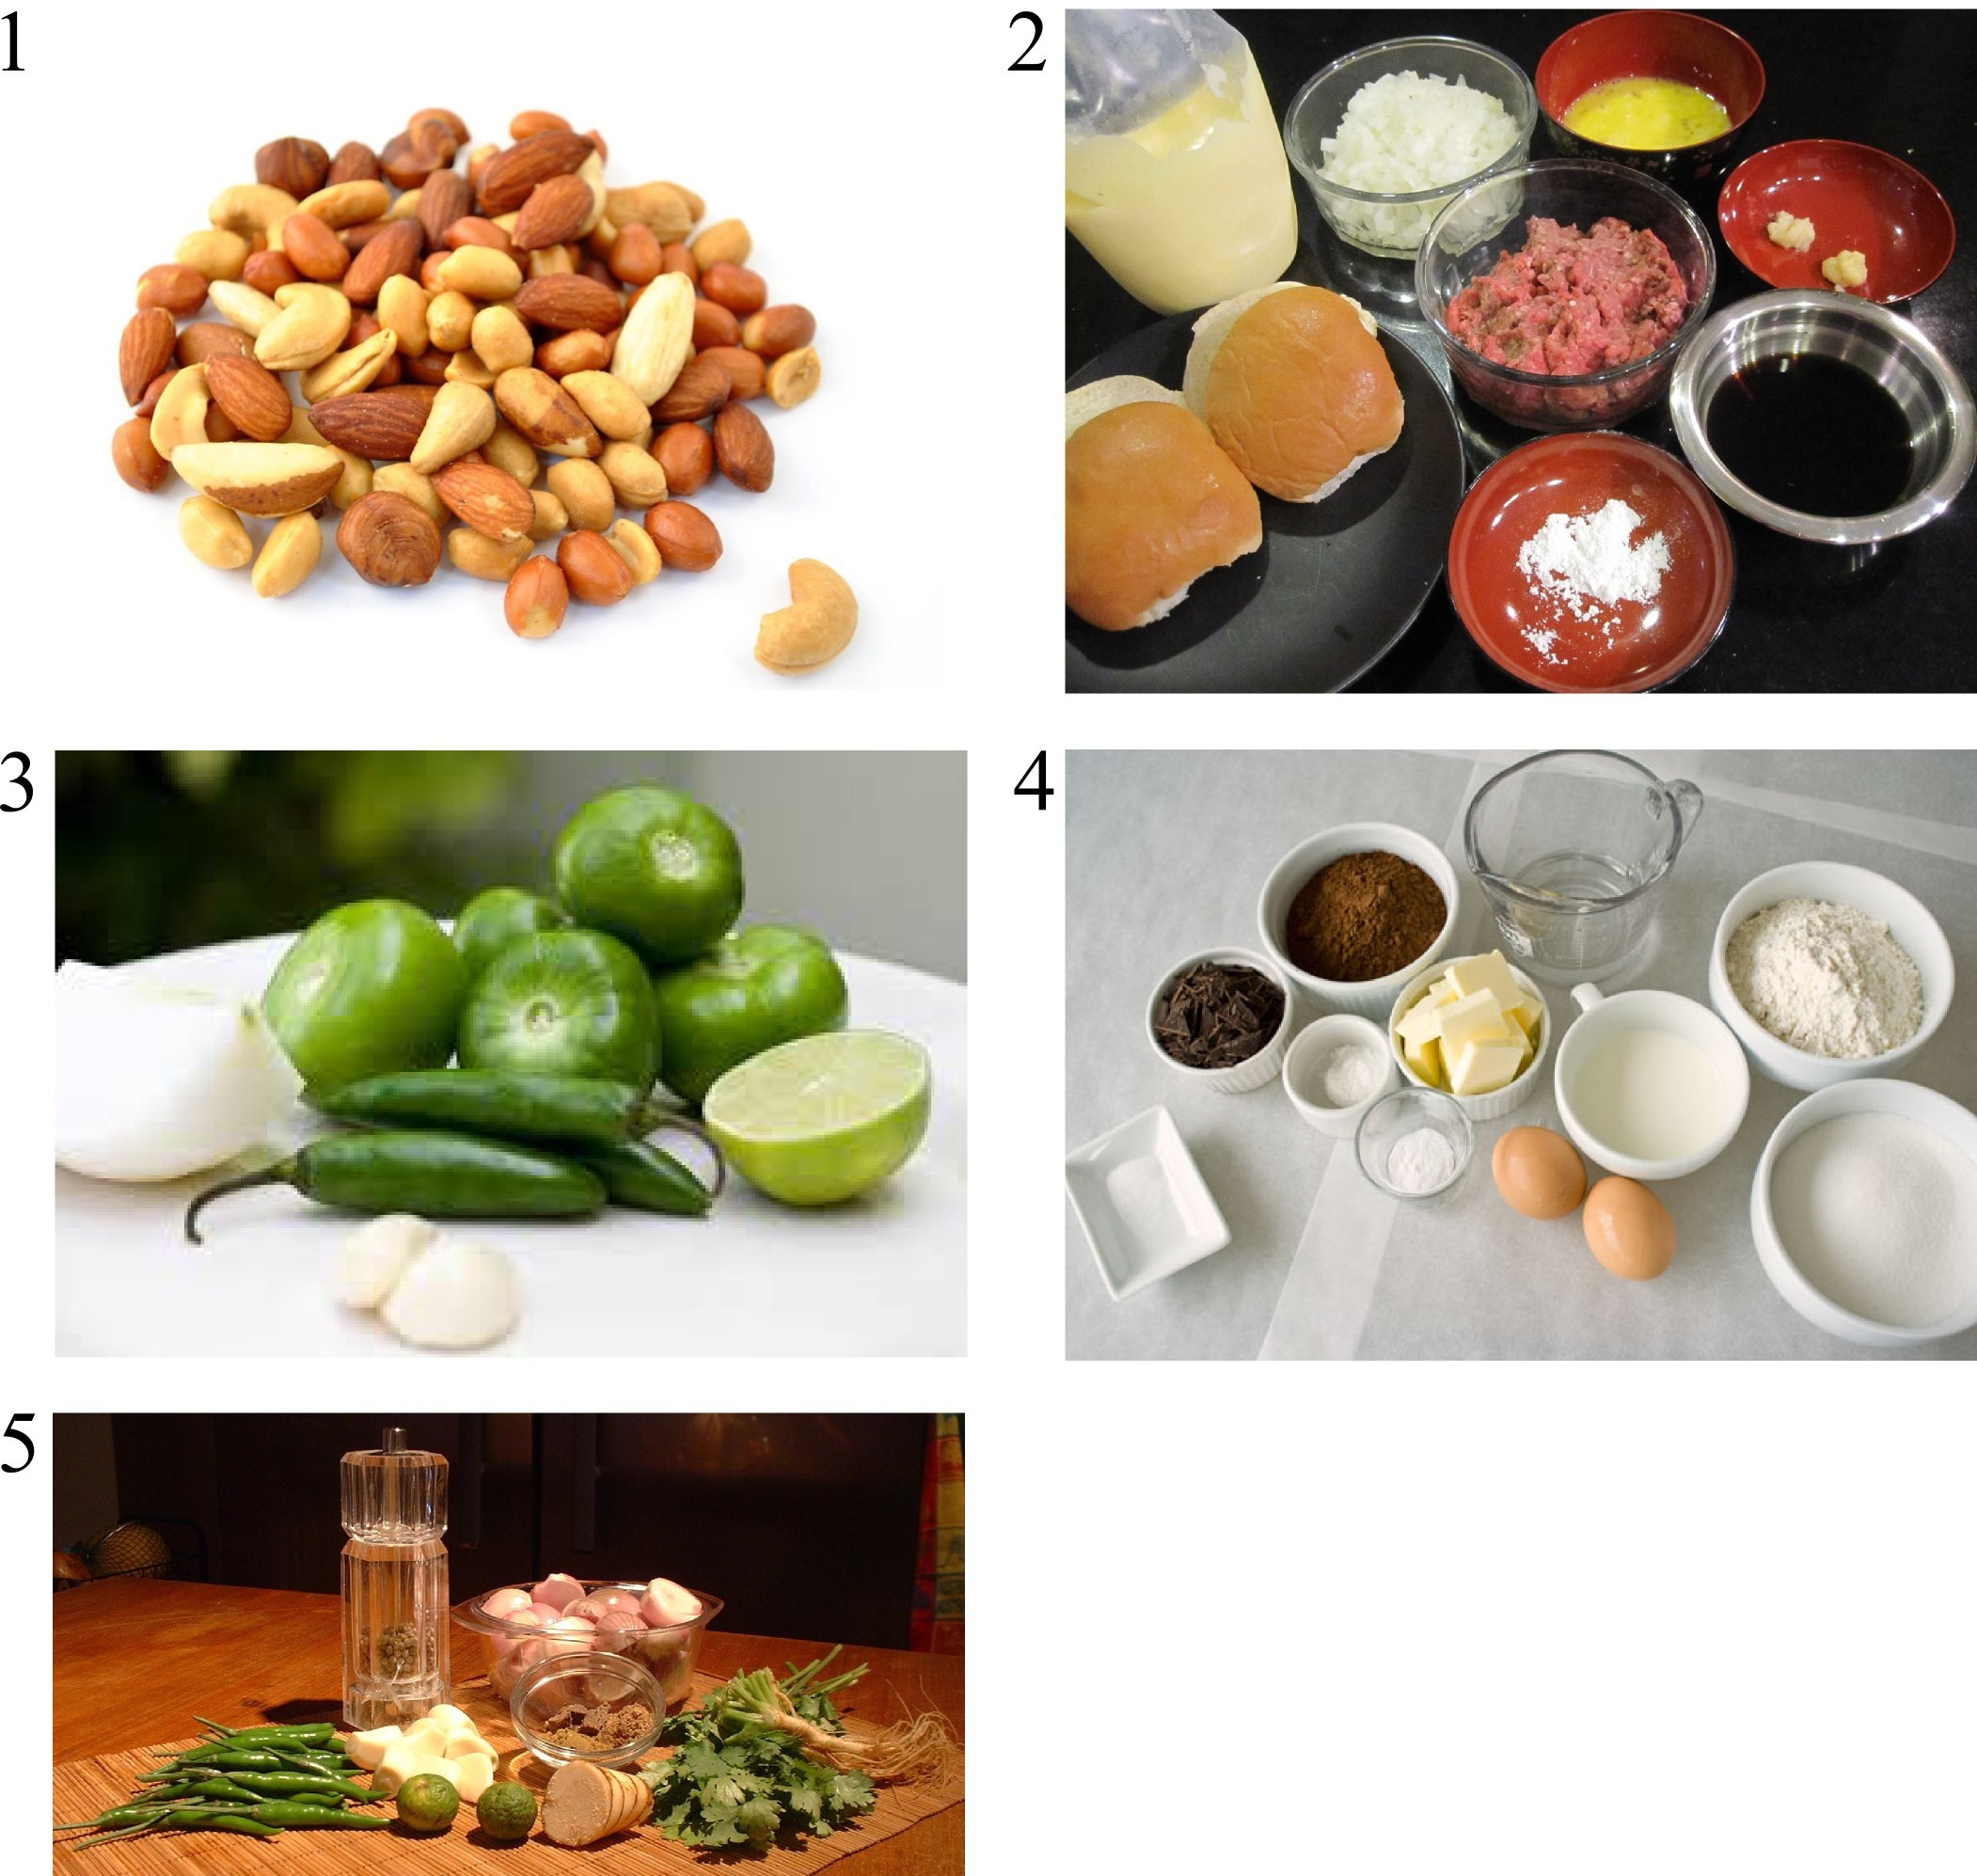
\includegraphics[scale=1.00]{figs/taskImages/ingredients.jpg}
	\caption*{Figure S4: Ingredients image set. These images were presented to workers 
		from certain treatments (see \textbf{Table 1}) in the main text.}
\end{figure*}

\end{document}


